\documentclass[10pt]{article}

\usepackage[utf8]{inputenc}
\usepackage[left=1.5cm,right=1.5cm]{geometry}
\usepackage[sfdefault]{noto}
\usepackage[T1]{fontenc}
\usepackage{hyperref}
\usepackage{graphicx}
\graphicspath{ {./resources/} }
\begin{document}

\title{\textbf{\underline{Projekt "Programmierung Neurales Netz" (Aufgabe 2)}}}
\author{\normalsize \textbf{Quellcode:} \url{https://github.com/11sepa1bif/JavaNeuralNet}}
\date{}
\maketitle

\section*{Implementierungsdetails}
\subsection*{Neurales Netz}
Ein \textbf{neurales Netz} besteht aus mindestens einem Input-/ und Outputlayer. Dazwischen befinden sich eine beliebige Anzahl Hidden Layer mit variabler Anzahl Neuronen. Während des Forward-Pass und der Backpropagation wird oft auf ein Layer eines bestimmten Indexes zugegriffen, daher scheint im ersten Moment ein Array sinnvoll. Gerade in Anbetracht der vielen Erweiterungs-/ und Optimierungsmöglichkeiten eines neuralen Netzes, die möglicherweise erst später im Entwicklungsprozess umgesetzt werden würden, erscheint eine ArrayList wegen ihrer fortgeschritteneren Konfiguration bzgl. ihrer Methoden, die die Klasse ArrayList implementiert, die ein normales Array nicht in diesem Ausmaß hat, sinnvoller. \newline
Ein \textbf{Layer} besteht aus einer festen Anzahl Neuronen. Da diese Anzahl bei der Initialisierung des Layers bereits fest steht und weniger komplexe Operation außer Schreib-/ und Lesezugriffe zu erwarten sind, wurde hier ein normales Array gewählt, das diese Neuronen enthält.\newline
Ein \textbf{Neuron} hat eine Anzahl eingehender Gewichte, die, da von einem voll vernetzten Netz ausgegangen wird, der Anzahl der Neuronen des vorherigen Layers entspricht. Da die Gewichte erst nach dem konstruieren aller Layer initialisiert werden, wurde auch hier auf die einfache Datenstruktur des Arrays gesetzt, da zu diesem Zeitpunkt alle Layer und somit auch die Anzahl der Neuronen des Vorgängerlayers bekannt ist. Außerdem hat ein Neuron einen Bias und einen Aktivierungswert, den Bias könnte man auch in einem Layer speichern, da dieser zu Beginn für alle Neuronen eines Layers gleich ist, allerdings verändern manche fortgeschrittenen Backpropagationalgorithmen auch diese Biases, weswegen es dennoch sinnvoll ist, diese in einem Neuron zu speichern. Deltas werden nicht gespeichert, da der implementierte Backpropagation-Algorithmus die Gewichte direkt verändert.

\subsection*{Initialisierung der Gewichte}
Die Gewichte können entweder zufällig über dem Intervall (-1.0; +1.0) oder nach dem Xavier Algorithmus initialisiert werden. Die Xavier Methode ist besonders effizient im Kombination mit der Sigmoid Aktivierungsfunktion, die hier verwendet wird und ist der zufälligen Initialisierung quasi immer überlegen.

\subsection*{Trainingsprozess}
Als Backpropagation Algorithmus wurde eine Erweiterung der Delta-Formel gewählt, die nicht erst die einzelnen Delta-Werte berechnet und nach einem weiteren Durchlauf erst die Werte aktualisiert, sondern die Werte werden direkt verändert, da dies die Komplexität und Laufzeit verbessert. Die Formel zur Aktualisierung der Gewichte ergibt sich aus der partiellen Ableitung des Fehlers nach dem Gewicht, das aktualisiert werden soll\footnote{\url{https://mattmazur.com/2015/03/17/a-step-by-step-backpropagation-example/}}.


\newpage

\section*{Konfiguration des Netzes durch den Nutzer}
\begin{figure}[htp]
\centering
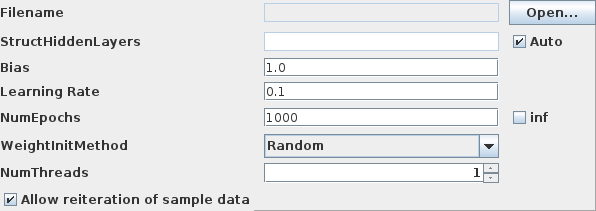
\includegraphics[scale=1.00]{settings.png}
\end{figure}

\noindent \textbf{Filename} Der Nutzer wählt eine Testdatei aus, die die zu lernenden Testdaten enthält, wobei eine Zeile einem Testdatensatz entspricht, die ersten beiden Spalten den Eingabewerten und die letzte Spalte der dichotomen Klassifizierungsmenge bestehend aus \{0,1\}. Die Klasse TestDataGenerator kann solche Testdaten generieren.\newline
\textbf{StructHiddenLayers} legt die Anzahl und Struktur der Hidden Layer in der Form x,y,z,... fest wobei x,y,z die Anzahl der Neuronen in der Hidden Layer Schicht in Position 1,2,3,... entspricht. "Auto" erstellt genau eine Hidden Layer Schicht mit der gleichen Anzahl von Neuronen wie die des Input-Layers (aktuell 2).\newline
\textbf{Bias} legt den Biaswert fest. Der Bias Wert wird aktuell nicht im Trainingsprozess verändert und bezieht sich auf alle Hidden Layer.\newline
\textbf{Learning Rate} Die Lernrate im Intervall (+0.0; +1.0).\newline
\textbf{NumEpochs} Die maximale Anzahl an Epochen, die der Lernprozess durchführen soll. "inf" entspricht einer unendlichen Anzahl von Epochen.\newline
\textbf{WeightInitMethod} Gibt an, wie die Gewichte initialisiert werden sollen (s.o.).\newline
\textbf{NumThreads} Mit wie vielen Threads der Trainingsprozess durchgeführt werden soll. Entspricht einem Wert in der Menge \{1,...,NUM\_CPUS\}, wobei NUM\_CPUS der Anzahl der Kerne bzw. Prozessor-Threads im Falle von Hyperthreading entspricht.\newline
\textbf{Allow reiteration of sample data} Legt fest, ob der gleiche Datensatz mehr als einmal trainiert werden darf. Hat eine höhere Priorität als "NumEpochs", um den gesamten Datensatz also genau einmal zu parsen sollte "NumEpochs" auf "inf" gesetzt und "Allow reiteration of sample data" nicht ausgewählt werden.

\newpage

\section*{Testergebnisse (Beispiel)}

\begin{figure}[htp]
\centering
\includegraphics[scale=0.60]{example2.png}
\end{figure}

\noindent Der Screenshot zeigt die Ausgabe des Programms über einem Testdatensatz mit 1000 Werten im Intervall [+0.0, +1.0] für x und y ohne Werte auf den Geraden x = 0.5 und y = 0.5, unterteilt in vier Quadranten die die XOR-Funktion simulieren sollen. Im Diagramm, das die gewichtete Fehlerquote über der Anzahl der Epochen darstellt, sieht man, das der Fehler mit zunehmender Anzahl Epochen abnimmt. Aus der Erfahrung mit anderen Testdurchläufen lässt sich sagen, dass die Qualität des Traininsgsprozesses sehr start von den konfigurierten Parametern abhängt und auch bei gleichen Parametern in verschiedenen Testdurchläufen start variiert. So hat sich gezeigt, dass in manchen Testdurchläufen der Fehler gegen verschiedene Werte konvergiert ist, die nicht null sind, was vermutlich am doch relativ simplen Backpropagation-Algorithmus liegt, der die Werte des Netzes auf ein Weise hin verändert, die bewirkt, dass diese sich entsprechend der Lernrate einem bestimmten Wert, einem (lokalen) Minimum annähern, das nicht unbedingt dem globalen Minimum entsprechen muss und dadurch nicht das bestmögliche Ergebnis produziert. In einer Verbesserung des Programms über den Rahmen dieses Projekts hinaus sollte also ein besserer Backpropagation-Algorithmus, wie z.B. Adam, implementiert werden. Außerdem sei anzumerken, dass ein Fehler von 0 für einen gegebenen Trainingsdatensatz vor dem Hintergrund des Overfitting nicht unbedingt erstrebenswert sein muss.

\end{document}